\documentclass[newPxFont]{beamer}
\usetheme{sthlm}
%\usecolortheme{sthlmv42}

%-=-=-=-=-=-=-=-=-=-=-=-=-=-=-=-=-=-=-=-=-=-=-=-=
%        LOADING PACKAGES
%-=-=-=-=-=-=-=-=-=-=-=-=-=-=-=-=-=-=-=-=-=-=-=-=
\usepackage[utf8]{inputenc}

\usepackage{chronology}

\renewcommand{\event}[3][e]{%
  \pgfmathsetlength\xstop{(#2-\theyearstart)*\unit}%
  \ifx #1e%
    \draw[fill=black,draw=none,opacity=0.5]%
      (\xstop, 0) circle (.2\unit)%
      node[opacity=1,rotate=45,right=.2\unit] {#3};%
  \else%
    \pgfmathsetlength\xstart{(#1-\theyearstart)*\unit}%
    \draw[fill=black,draw=none,opacity=0.5,rounded corners=.1\unit]%
      (\xstart,-.1\unit) rectangle%
      node[opacity=1,rotate=45,right=.2\unit] {#3} (\xstop,.1\unit);%
  \fi}%

%-=-=-=-=-=-=-=-=-=-=-=-=-=-=-=-=-=-=-=-=-=-=-=-=
%        BEAMER OPTIONS
%-=-=-=-=-=-=-=-=-=-=-=-=-=-=-=-=-=-=-=-=-=-=-=-=

%\setbeameroption{show notes}


%-=-=-=-=-=-=-=-=-=-=-=-=-=-=-=-=-=-=-=-=-=-=-=-=
%
% PRESENTATION INFORMATION
%
%-=-=-=-=-=-=-=-=-=-=-=-=-=-=-=-=-=-=-=-=-=-=-=-=

\title{OnlineATPs}
\subtitle{A client for the TPTP World}
% \date{\small{\jobname}}
\date{\today}
\author{By Jonathan Prieto-Cubides\\
Supervisor: Andr\'es Sicard-Ram\'irez}
\institute{
Logic and Computation Research Group\\
EAFIT University\\
Medell\'in, Colombia
}
\hypersetup{
pdfauthor = {Jonathan Prieto-Cubides: jprieto9@eafit.edu.co},
pdfsubject = {ATP},
pdfkeywords = {ATPs, OnlineATPs},
pdfmoddate= {D:\pdfdate},
pdfcreator = {}
}

\begin{document}
\maketitle

% \section*{Overview}
\begin{frame}{Overview}
% For longer presentations use hideallsubsections option
\tableofcontents[hideallsubsections]
\end{frame}



\section{The tool}

\begin{frame}{Abstract}
OnlineATPs is a command-line tool for connect to the web service SystemOnTPTP of the TPTP World.
This new tool allows us to use ATPs without installing any of them. We can install it on Linux, Windows or Mac.
With OnlineATPs you are capable to test a problem against at least sixty ATPs, check for unsatisfability, get some proofs and others functions.
\end{frame}

\begin{frame}{Overview}

\onlineatps connects to \alert{\systemontptp} and allows us to take
advantage of using \alert{\atps} \textbf{without installing} any of them.
\begin{itemize}
\item Is an open source project located on \shell{Github}.
\begin{itemize}
  \item You are free to contribute, fork, everything.
  \item Indeed, now there are some issues open.
  \end{itemize}
\item Is a software written on \shell{Haskell}
\begin{itemize}
  \item Tested with \texttt{GHC 7.6.3, 7.8.4, 7.10.3, 8.0.1}.
  \end{itemize}
\item Is a command-line application cross-platform:
\begin{itemize}
  \item OSX, Linux, Windows.
\end{itemize}
\item \apia has full support for \onlineatps.
\end{itemize}
\end{frame}

\begin{frame}
\systemontptp is a website and interface for solving problems using \atps.
The url address is \url{www.cs.miami.edu/~tptp/cgi-bin/SystemOnTPTP}.\\
Other services you can find there:
\begin{itemize}
\item TPTP Library of Problems.
\item SystemB4TPTP for prepare problems.
\item SystemOnTSTP to process solutions.
\end{itemize}
\end{frame}

\begin{frame}
\begin{block}{Keywords of the project}
\begin{itemize}
\item \atp Systems
\item \keyword{TPTP} World
\item \systemontptp interface
\item Theorem proving
\end{itemize}
\end{block}
\end{frame}


\begin{frame}{Automatic Theorem Provers}
\emph{Automated Theorem Proving} deals with the development
 of computer programs that show that some statement
 -the conjecture- is a logical consequence of a set
 of statements -the axioms and hypotheses-\footnote{
 \url{http://www.cs.miami.edu/~tptp/OverviewOfATP.html}}.

\begin{equation}
\label{ATPs:1}
{A_{1}, A_{2}, \cdots,A_n} \stackrel{?}{\vDash} C.
\end{equation}

\atp systems are used in a wide variety of domains.\\
Examples: logic, mathematics, computer science, engineering, and social science.
\end{frame}


\begin{frame}[fragile]{Automatic Theorem Provers}
\begin{table}[!ht]
\centering
\caption{Some \atps for PROP, FOF, and HOL}
\newcolumntype{A}{>{\tt}c}
\scalebox{0.75}{
\begin{tabular}[!ht]{|A|c|c|c|c|c|c|c|}
\hline
\textbf{ATP}      & \textbf{Version} & \textbf{Update} & \textbf{PROP} & \textbf{FOF}  & \textbf{SMT 2.0} &
\textbf{\texttt{TPTP} In} & \textbf{\texttt{TSTP} Out} \\ \hline
\label{ATP:cvc4}\href{http://cvc4.cs.nyu.edu/web/}{CVC4}  &1.4 &15/07/14 &$\checkmark$ &$\checkmark$ &$\checkmark$ &$\checkmark$ &- \\ \hline
\label{ATP:eprover} \href{http://www.eprover.org/}{\keyword{EProver}}  &1.9 &14/7/15 &$\checkmark$ &$\checkmark$ &-  &$\checkmark$ &$\checkmark$  \\ \hline
\label{ATP:equinox}\href{https://github.com/nick8325/equinox}{Equinox}  &6.0.1 &5/7/12 &$\checkmark$ &$\checkmark$  &-  &$\checkmark$ &- \\ \hline
\label{ATP:iprover}\href{https://code.google.com/archive/p/iprover/}{iProver}  &0.8.1 &-/-/10 &$\checkmark$ &$\checkmark$  &$\checkmark$ &$\checkmark$ &- \\ \hline
\label{ATP:ileancop}\href{http://www.leancop.de/}{leanCoP} &2.1 &1/1/15 &$\checkmark$ &$\checkmark$  &- &$\checkmark$ &-$^*$ \\ \hline
\label{ATP:metis}\href{http://www.gilith.com/software/metis/}{\keyword{Metis}}    &2.3 &9/11/10 &$\checkmark$ &$\checkmark$ &-   &$\checkmark$ &$\checkmark$ \\ \hline
\label{ATP:prover9}\href{https://www.cs.unm.edu/~mccune/mace4/}{Prover9}  &2009-11A  &4/11/09 &$\checkmark$ &$\checkmark$  &-  &-$^*$ &- \\ \hline
\label{ATP:spass}\href{http://www.spass-prover.org/download/index.html}{SPASS}    &3.7 &23/02/10 &$\checkmark$ &$\checkmark$   &-  &$\checkmark$ &- \\ \hline
\label{ATP:vampire}\href{http://www.vprover.org/}{\keyword{Vampire}}  &2.6 &-/-/11 &$\checkmark$ &$\checkmark$   &- &$\checkmark$ &$\checkmark$ \\ \hline
\label{ATP:z3}\href{https://github.com/Z3Prover/z3}{Z3}  &4.4.1 &5/10/15 &$\checkmark$ &$\checkmark$   &$\checkmark$ &- &- \\ \hline
\end{tabular}
}
\end{table}
\end{frame}


\begin{frame}[fragile]{Installing one \atp }
Did you try installing some \atp before with success at first try?\\
\begin{itemize}
\item \keyword{EProver}
  \begin{lstlisting}
  $ cd ~
  $ wget http://wwwlehre.dhbw-stuttgart.de/~sschulz/WORK/E_DOWNLOAD/V_1.9.1/E.tgz
  $ tar -xzf E.tgz
  $ cd E
  $ ./configure --bindir=~/bin
  $ make
  $ make install
  \end{lstlisting}
\end{itemize}
\end{frame}

\begin{frame}
\begin{itemize}
\item Done! And if you want to install more than one or three \atps?\\
\item Did you try installing with \spass, \metis, \vampire?\\
\item Installation failures?
\item Instead you can install \onlineatps!
\end{itemize}
\end{frame}

\begin{frame}[fragile]{Installing \onlineatps}
\begin{itemize} \onlineatps
\begin{lstlisting}
$ git clone https://github.com/jonaprieto/online-atps
$ cd ~/online-atps
$ cabal install
\end{lstlisting}
\item In the future
\begin{lstlisting}
$ cabal install online-atps
\end{lstlisting}
\end{itemize}
\end{frame}

\begin{frame}

About the I/O of \atps
\begin{itemize}
\item Input files
\item Output files
\end{itemize}

\end{frame}


\begin{frame}[fragile]{The input format for some ATPs}
\keyword{TPTP} is a standard format to
write problems in different formalisms like
first order logic or high order logic.

\begin{lstlisting}
$ cat basic.tptp
fof(a1, axiom, a).
fof(a2, axiom, b).
fof(a3, axiom, (a & b) => z).
fof(a4, conjecture, z).
\end{lstlisting}

\end{frame}


\begin{frame}[fragile]{The theorem}

\begin{theorem} $\{a, b, a\wedge b \rightarrow z\} \vdash z$
\label{prob1}
\end{theorem}

\begin{proof}
Natural deduction proof.\hfill
\label{basic-der}
\begin{prooftree}
\AxiomC{$a$}
\AxiomC{$b$}
\RightLabel{\scriptsize($\wedge$-{\bfseries intro})}
\BinaryInfC{$a\wedge b$}
\AxiomC{$a\wedge b\rightarrow z$}
\RightLabel{\scriptsize($\rightarrow$-{\bfseries Elim})}
\BinaryInfC{z}

\RightLabel{\scriptsize($\rightarrow$-{\bfseries Intro})}
\UnaryInfC{$(a\wedge b \rightarrow z) \rightarrow z$}
\end{prooftree}
\end{proof}
\end{frame}


\begin{frame}[fragile]{Using EProver to get an answer}
The output from the problem later using \eprover.
\begin{lstlisting}
$ eprover --auto --tptp3-format basic.tptp
# Proof found!
# SZS status Theorem
\end{lstlisting}
\end{frame}


\begin{frame}
\frametitle{Using a nice feature of Eprover}
\eprover can output a graph (.dot format) of the proof.
\begin{figure}[h!]
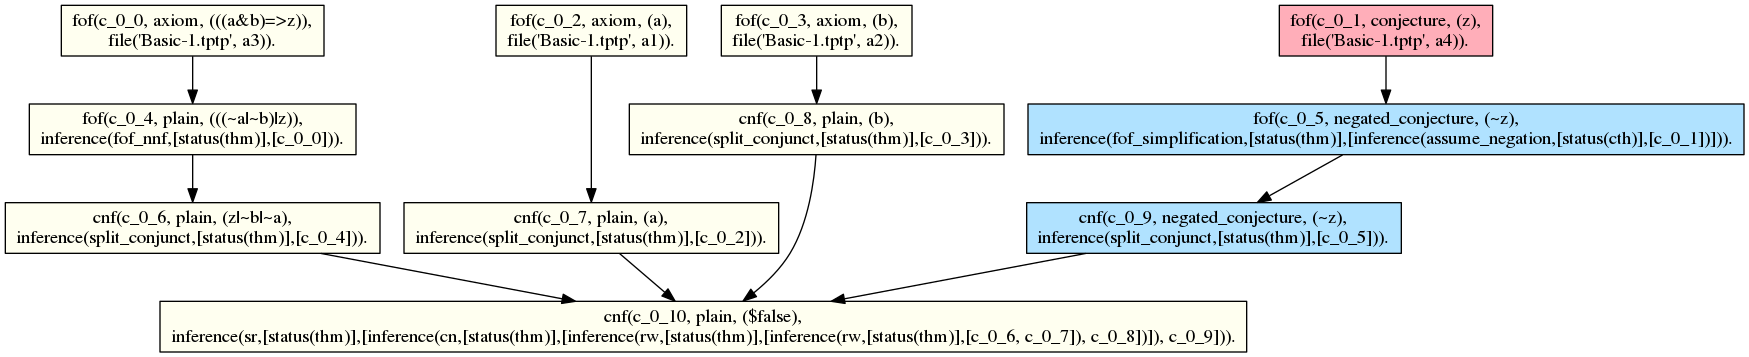
\includegraphics[scale=0.18]{graphproof}
\caption {Proof graph of the threorem \ref{prob1} }
%\label{Figure 8}
\end{figure}
\end{frame}


\begin{frame}{The Output Format}
A few \atps use \keyword{TSTP} format.
\begin{table}
\label{table:1}
\centering
\caption{Some examples of outputs when an ATP finishes successfully}
\vspace*{1.5mm}
\newcolumntype{A}{>{\tt}c}
\scalebox{0.7}{
\begin{tabular}{|A|c|l|}\hline
\textbf{ATP} &\textbf{Version Tested} &\textbf{Sucess} \\ \hline
\cvc &1.4 &\lstinline!SZS status Theorem!\\ \hline
\eprover &1.9 &\lstinline!Proof found! \\ \hline
\equinox &5.0alpha &\lstinline!+++ RESULT: Theorem! \\ \hline
\ileancop &1.3 beta1 &\lstinline!Intuitionistic Theorem! \\ \hline
\metis &2.3 &\lstinline!SZS status Theorem! \\ \hline
\spass &3.7 &\lstinline!Proof found!  \\ \hline
\vampire &0.6 &\lstinline!Termination reason: Refutation! \\ \hline
\z &4.4.1 &\lstinline!unsat!\\ \hline
\end{tabular}
}
\end{table}
\end{frame}

\begin{frame}{Future work}
\begin{itemize}
\item We want to give full support for all features of TPTP World.
\begin{itemize}
  \item Customize the command arguments that you send for each \atps.
  \item Recommend Systems.
\end{itemize}
\item More features focus on \apia needs.
\item YAML Configure files.
\item Asyncronic calls.
\end{itemize}
\end{frame}


% % \begin{frame}[fragile]{\tptp standard form}

% % \end{frame}

% % \begin{frame}[fragile]{\tptp standard form}

% % \label{syntax:fof}
% % \begin{grammar}
% % <cnf_annotated> ::= \textbf{cnf}(<name>,<formula_role>,<cnf_formula>,<annotations>).

% % <fof_annotated> ::= \textbf{fof}(<name>,<formula_role>,<fof_formula>,<annotations>).
% % \end{grammar}
% % \end{frame}

% % \begin{frame}
% % \begin{grammar}
% % <name> ::= <atomic_word> | <integer>

% % <formula_role> ::= {\bf axiom} | hypothesis | definition | assumption
% % \alt lemma | theorem | corollary | {\bf conjecture}
% % \alt {\bf negated_conjecture} | {\bf plain }| type | unknown
% % \end{grammar}
% % \end{frame}

% % % \begin{frame}[fragile]{TSTP format for solution}
% % % \scalebox{0.6}{
% % % \begin{lstlisting}[label=bash:eprover2, caption=An excerpt from the derivation of the problem \ref{prob1} using the tool of \eprover]
% % % $ eproof --tptp3-format basic-1.tptp
% % % # Problem is unsatisfiable (or provable), constructing proof object
% % % # SZS status Theorem
% % % # SZS output start CNFRefutation.
% % % fof(1, axiom,a,file('basic-1.tptp', a1)).
% % % fof(2, axiom,b,file('basic-1.tptp', a2)).
% % % fof(3, axiom,((a&b)=>z),file('basic-1.tptp', a3)).
% % % ...
% % % cnf(15,negated_conjecture,($false),inference(rw,[status(thm)],[11,14])).
% % % cnf(16,negated_conjecture,($false),inference(cn,[status(thm)],[15])).
% % % cnf(17,negated_conjecture,($false),16,['proof']).
% % % \end{lstlisting}
% % % }
% % % \end{frame}





\subsection{Inside the Code}

\begin{frame}[c]{Modules}
Let's check some challenges inside the code!
\begin{block}{Modules available}
\begin{itemize}
\item \shell{OnlineATPs.CheckOutput}
\item \shell{OnlineATPs.Consult}
\item \shell{OnlineATPs.Options}
\item \shell{OnlineATPs.SystemATP}
\item \shell{OnlineATPs.SystemOnTPTP}
\item \shell{OnlineATPs.Urls}
\item \shell{OnlineATPs.Utils.Yaml}
\end{itemize}
\end{block}
\end{frame}


\bibliography{biblio}
\end{document}
